\section{Feature detection}
\label{sec:sec2_feature_detection}

In the context of computer vision and image processing, image features are distinctive landmarks in the images, preferably unsusceptible to point-of-view, scale, and the aperture problem. Features are important as they provide information on the image, which can be used for recognition, matching, reconstruction, and tracking, among many other applications. Many types of features can be considered, such as edges, corners, blobs, ridges, and shapes.

The process of identifying features in an image is called feature detection, and multiple detectors have been described in the literature, dependent on the features of interest, such as Canny and Sobel detectors (for edges), Hough transform (for shapes), Laplacian operator (for blobs), and Harris detector (for corners).

For event-based cameras, new types of features, as well of detectors, are being proposed, as classical techniques are not easily transferable in most cases, or result in a non-negligible performance decrease, due to conversion overhead from asynchronous events to frames. However, corners seem to prove as interesting features to use, as not only can they be used to match features between the event stream and full frame images, allowing for sensor fusion, native event algorithms are available, which leverage the potential of events, namely speed and event independence.

\subsection{Classic corner detection}
\label{sec:sec2_classic_corner_detection}

The typical example for a classic corner detector is the Harris Corner Detector (\cite{harris1988combined}). It works using the following steps:

\begin{itemize}
    \item Compute the x-wise $I_x(x,y)$ and y-wise $I_y(x,y)$ partial image derivatives
    \item Compute the second-order derivatives $I_x^2(x,y)$  and $I_y^2(x,y)$, and cross-derivatives $I_x I_y(x,y)$
    \item Compute the second-moment matrix $M(x,y)$
    \item Compute the Harris score
    \item Detect local extrema whose Harris score is greater than the set threshold
\end{itemize}

The partial derivatives are computed by applying a Sobel derivative kernel (usually 3x3 or 5x5 kernels) to the whole image, producing the x-wise $I_x (x,y)$ and y-wise $I_y (x,y)$ partial image derivatives. From these derivatives, we can define the vector $\nabla I(x,y) = (I_x (x,y),I_y (x,y))^T$ and the second-moment matrix for each pixel ($M(x,y)$), defined as $M(x,y)= \sum_{(x,y)\in patch}^{}g(x,y)\nabla I(x,y)\nabla I^T(x,y)$, where $g(x,y)$ is a Gaussian weighting function centred around $(x,y)$, which controls the “sharpness” of the edge.

Then, we can compute the Harris score as defined in Eq.\,\eqref{eq:sec2_harris_score}.

\begin{equation}
    \label{eq:sec2_harris_score}
    H(x,y)=\lambda_1\lambda_2-k\times \left( \lambda_1 + \lambda_2 \right)^2 = det(M) - k\times trace (M)^2
\end{equation}

Where $k$ is an empirical value, $k \in \left[ 0.04; 0.06 \right ]$.

Finally, if $H(x,y)\geq H_0$, we consider the pixel as a corner. This will produce corner blobs. In order to select a single pixel to represent the corner, we select the local extrema (the pixel with the highest Harris score).

Another option to evaluate the presence of corners is to analyse the eigenvalues of M. If both eigenvalues are low, no interesting features are detected. If one is low, but the other is high, we are in the presence of and edge. Lastly, if both eigenvalues are high, the pixel is likely a corner. As such, one interpretation of the Harris detector is that corners are identified by finding the intersection of edges.

With this in mind, an alternative for the corner analysis, is to check the value of the lowest eigenvalue of $M (\lambda_{min})$, through the approximation Eq.\,\eqref{eq:sec2_min_eig}.

\begin{equation}
    \label{eq:sec2_min_eig}
    \lambda_{min} \approx \frac{\lambda_1\lambda_2}{\lambda_1+\lambda_2}=\frac{det(M)}{trace(M)}
\end{equation}

And then this value is used as a corner criterion.

\subsection{Event-based corner detection}
\label{sec:sec2_event_corner}

Due to the nature of events, gradient operators are not possible (at least directly applied to the event stream), since there is no image on which to apply them, and multiple techniques have been proposed, of which three will be presented.

\subsubsection{Space-time detection}
\label{sec:sec2_space_time}

This method relies on the space-time properties of events, and creates a 3D representation, containing the spatial position of an event $(x,y)$, as well as the time it was received. In this representation, edges moving with uniform linear speed create planes (stack of lines at different instants), and corner movement creates lines (stack of points at different instants).

As such, this technique tracks moving edges by fitting planes in this 3D representation, implicitly estimating the speed of the moving edge (optical flow). Each new event is matched to the previously estimated planes, and the estimates are updated, as shown in Fig.\,\ref{fig:sec2_plane_distance}. 

\begin{figure}[ht]
    \centering
    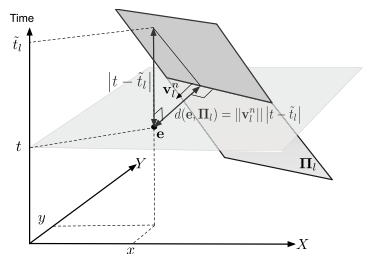
\includegraphics[width = 0.5\linewidth]{distance.png}
    \caption[Distance calculation from event to plane, and plane fitting]{Distance calculation from event to plane, and plane fitting, from \cite{clady2015asynchronous}}
    \label{fig:sec2_plane_distance}
\end{figure}

The way this technique identifies (and tracks corners) is by detecting intersection between these planes, as these intersections correspond to the corner movement through a period of time (Fig.\,\ref{fig:sec2_corner_spacetime}).

\begin{figure}[ht]
    \centering
    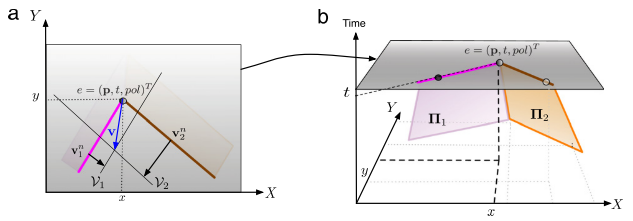
\includegraphics[width = 0.5\linewidth]{corner_spacetime.png}
    \caption[Corner detection using spacetime approach]{Corner are the result of the intersection of lines (edges) at a given timestamp, which themselves result from the spacetime planes that are being estimated, from \cite{clady2015asynchronous}}
    \label{fig:sec2_corner_spacetime}
\end{figure}

\subsubsection{Event-based Harris Corner Detector}
\label{sec:sec2_event_harris}

This technique (from \cite{vasco2016fast}) relies on the Surface of Active Events (SAE), a representation system for events, which keeps track of the timestamp of the most recent event for any given pixel, regardless of polarity, defined by Eq.\,\ref{eq:sec2_sae}. Indeed, it is a spatial representation ($(x,y)$ coordinates, corresponding to each pixel), which can be discretized by assigning a value to each pixel based on its timestamp. Fig.\,\ref{fig:sec2_sae} shows an example of the SAE, where the events are represented from white to grey, as they go from more recent to older.

\printglossaries


\begin{equation}
    \label{eq:sec2_sae}
    SAE:(x,y) \to t
\end{equation}

\begin{figure}[ht]
    \centering
    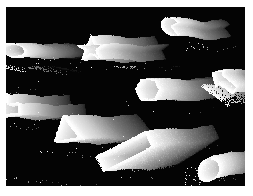
\includegraphics[width = 0.5\linewidth]{sae.png}
    \caption[Representation of the Surface of Active Events (SAE)]{Representation of the Surface of Active Events (SAE), with more recent events being represented in a stronger white, from \cite{mueggler2017fast}}
    \label{fig:sec2_sae}
\end{figure}

Since this discretized representation is now a frame in the classical sense, we can apply the Harris Corner Detector directly to the SAE and identify the corners from these results. 
A more efficient implementation relies on considering only the neighbouring region of an event as it arrives, instead of the whole SAE. As such, only a subset of the SAE is analysed. Since each event, and consequently, each subset, is independent on the other subsets (provided the subsets do not overlap), parallel implementations are possible, and also improve speed.

\subsubsection{SAE-based corner detector}
\label{sec:sec2_sae_corner_detection}


This technique also relies on the SAE representation of events but does not perform any computations. Rather, it performs only comparison operations on a local neighbourhood around the relevant event.

As each event is received, its timestamp is compared with the neighbouring pixels using circular segments (for isotropic response and efficiency), and checked if patterns similar to the one in Fig.\,\ref{fig:sec2_sae_corner} are present (contiguous pixels with decreasing timestamps), as these are typical corner patterns.

Though this method is not as effective, it is much faster, as no computations are performed, and each event can be processed independently (and concurrently in a parallel fashion).

\begin{figure}[ht]
    \centering
    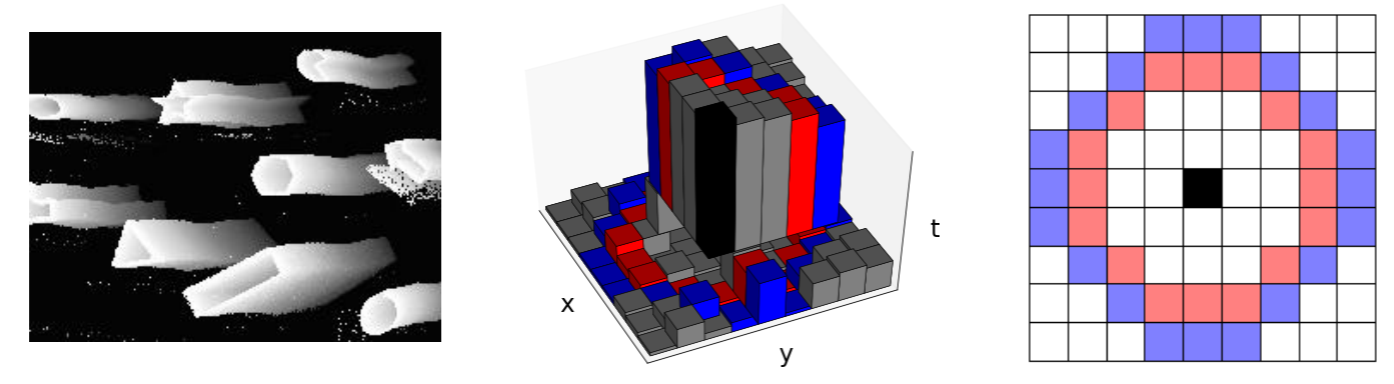
\includegraphics[width = 0.5\linewidth]{sae_corner.png}
    \caption[Corner detection through SAE]{(a) Representation of SAE, on which the comparison filter from (c) is applied, and checked for patterns of decreasing intensity from centre to surrounds, as shown in (b), from \cite{mueggler2017fast}}
    \label{fig:sec2_sae_corner}
\end{figure}
